\chapter{Teoria dei Grafi}
\begin{flushleft}
    \textbf{Grafo}: si dice \textbf{grafo} una coppia ordinata $G=(V,E)$, con $V$ \textbf{insieme dei vertici} ed $E$ \textbf{insieme degli spigoli}, tali che $E \subseteq \binom{V}{2}$ (cioè che tutti gli elementi di $E$ devono essere delle coppie, ossia di \textit{cardinalità} 2).
    
    \begin{figure}[h]
        \centering
        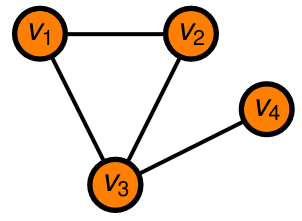
\includegraphics[width=0.25\textwidth]{img/grafi_1}
    \end{figure}

    {\centering
        $V = \{v_1, v_2, v_3, v_4\}$ \\
        $E = \{\{v_1, v_2\}, \{v_2, v_3\}, \{v_3, v_1\}, \{v_3, v_4\}\}$
    \par}
    \begin{itemize}[nosep]
        \item \textbf{vertici adiacenti}: dato un grafo $G=(V, E)$, si dice che $v$ e $w$, con $v, w \in V$, sono \textit{adiacenti} su $G$ se $\exists\{v,w\} \in E$, ovvero 2 vertici $v,w$ si dicono adiacenti se, nell'insieme $E$, esiste la coppia che contiene quei due vertici.
        \item \textbf{vertici estremi}: se $e=\{v, w\} \in E$ si dice che lo spigolo $e$ ha come \textit{estremi} i vertici $v, w \in V$.
        \item \textbf{grafo orientato}: se le coppie di $E$ sono ordinate $(\{v, w\} \neq \{w, v\})$.
        \item \textbf{loop o cappio}: se uno spigolo ha due estremi coincidenti allora si parla di \textbf{pseudografo}.
        \item \textbf{spigoli multipli}: Se $E$ è un \textit{multinsieme} (ovvero i suoi elementi possono essere ripetuti), allora il grafo prende il nome di \textbf{multigrafo}. Al suo interno, più spigoli con gli stessi estremi si dicono \textit{spigoli multipli}.
        \newpage
        \item \textbf{matrice delle adiacenze}: dato un grafo $G=(V, E)$ finito (ovvero con cardinalità di $V$ finita) tale che $V = \{v_1, v_2, ..., v_n\}$ definiamo \textbf{matrice di adiacenza} la matrice $A = (a_j^i)$, con $i,j \in \mathbb{N}_n$ in cui:

        {\centering
            \begin{minipage}[t]{0.45\textwidth}
                \centering
                $a_i^j = \begin{cases} 1 \quad \text{se} \; \exists \{v_i, v_j\} \in E \\
                0 \quad \text{altrimenti} \end{cases}$
            \end{minipage}
            \hfill
            \begin{minipage}[t]{0.45\textwidth}
                \centering
                $A = \left(\begin{array}{cccc} 0 & 1 & 1 & 0 \\
                    1 & 0 & 1 & 0 \\
                    1 & 1 & 0 & 1 \\
                    0 & 0 & 1 & 0 \end{array}\right)$
            \end{minipage}
        \par}
    \end{itemize}
\end{flushleft}

\section{Grafi Notevoli}
\begin{flushleft}

    \textbf{Grafo cammino con $n$ vertici} ($P_n (n \in \mathbb{N})$): $V = \{v_1, v_2, ..., v_n\}$ e $\{\{v_i, v_{i+1}\} \; | \; i \in \mathbb{N}_{n-1}\}$

    \begin{figure}[h]
        \centering
        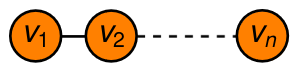
\includegraphics[width=0.25\textwidth]{img/grafo_cammino}
    \end{figure}

    \textbf{Grafo ciclo su $n$ vertici} ($C_n (n \in \mathbb{N})$): $V = \{v_1, v_2, ..., v_n\}$ e $E = \{\{v_i, v_{i+1}\} \; | \; i \in \mathbb{N}_{n-1}\} \cup \{v_n, v_1\}$
    
    \begin{figure}[h]
        \centering
        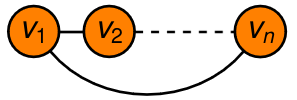
\includegraphics[width=0.25\textwidth]{img/grafo_ciclo}
    \end{figure}

    \textbf{Grafo completo su $n$ vertici} ($K_n (n \in \mathbb{N})$): $V = \{v_1, v_2, ..., v_n\}$ e $E = \{\{v_i, v_{i+1}\} \; | \; i, j \in \mathbb{N}_n \; \text{con} \; i \neq j\} = \binom{V}{2}$

    \begin{figure}[h]
        \centering
        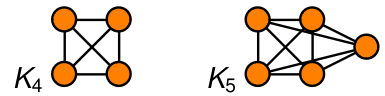
\includegraphics[width=0.35\textwidth]{img/grafo_completo}
    \end{figure}

    \textbf{Grafo completo bipartito di tipo $(n, m)$} ($K_{(n, m) \in \mathbb{N}^2}$): V in questo caso è composto da 2 tipologie di vertici ($V = \{v_1, ..., v_n\} \cup \{w_1, ..., w_m\}$), mentre gli spigoli vanno da un gruppo di vertici all'altro, con tutte le possibili combinazioni: $E = \{\{v_i, w_j\} \; | \; i \in \mathbb{N}_n, \; j \in \mathbb{N}_m\}$

    \begin{center}
        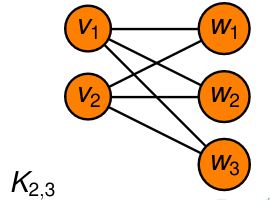
\includegraphics[width=0.2\textwidth]{img/grafo_com_bip}
    \end{center}
\end{flushleft}

\newpage
\begin{flushleft}

    \textbf{Grafo Bipartito}: un grafo $G = (V, E)$ si dice \textit{bipartito} se:

    {\centering
        $V = V' \cup V''$, $V' \cap V'' = \emptyset$ \\
        $\forall e = \{v, w\} \in E \; \Rightarrow \; v \in V', \; w \in V''$
    \par}
    ovvero se tutti gli spigoli hanno un vertice in un insieme e uno nell'altro.

    \begin{figure}[h]
        \centering
        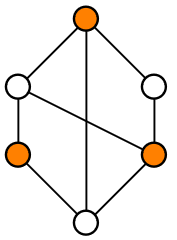
\includegraphics[width=0.15\textwidth]{img/grafo_bip}
    \end{figure}

\end{flushleft}

\section{Isomorfismo tra grafi}

\begin{flushleft}

    \textbf{Morfismo}: si dice \textit{morfismo} tra due grafi $G = (V, E)$ e $G' = (V', E')$ se esiste un'applicazione $f: V \mapsto V'$ tale che:

    {\centering
        $\forall e = \{v, w\} \in E, \exists e' = \{f(v), f(w)\} \in E'$
    \par}

    \textbf{Isomorfismo}: due grafi $G = (V, E)$ e $G' = (V', E')$ si dicono \textit{isomorfi} se esiste un'applicazione \textbf{biiettiva} $f: V \mapsto V'$ tale che si $f$ che la sua inversa $f^{-1}$ siano \textbf{morfismi}:

    {\centering
        $e = \{v, w\} \in E \; \Leftrightarrow \; e' = \{f(v), f(w)\} \in E'$
    \par}
    In pratica, 2 grafi sono isomorfi se uno è ottenibile dall'altro solo rinominando i vertici.

    \begin{figure}[h]
        \centering
        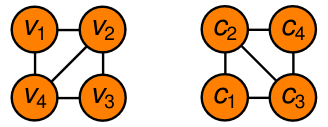
\includegraphics[width=0.35\textwidth]{img/isomorfismo}
        \caption{Coppia di Grafi Isomorfi}
        \label{fig:isomorfismo}
    \end{figure}
    \textbf{N.B.}: l'isomorfismo tra grafi è una \textbf{relazione di equivalenza}, dalla quale ottengono quante sono le classi di equivalenza rispetto all'isomorfismo tra grafi: 

    {\centering
        $g_n = \# \frac{\mathcal{G}_n}{\cong}$
    \par}
    dove $\mathcal{G}_n$ è l'insieme di tutti i grafi con $n$ vertici. Nella Fig. \ref{fig:isomorfismo} è possibile costruire un'applicazione biunivoca $f: V(G) \mapsto V'(G')$ tale che:

    {\centering
        \begin{minipage}[t]{0.45\textwidth}
            \centering
            $v_1 \mapsto c_1$ \\
            $v_2 \mapsto c_2$ \\
        \end{minipage}
        \begin{minipage}[t]{0.45\textwidth}
            \centering
            $v_4 \mapsto c_3$ \\
            $v_3 \mapsto c_4$
        \end{minipage}
    \par}
\end{flushleft}

\begin{flushleft}

    \textbf{Teorema}:

    {\centering
        $\frac{n^2}{2}(1 - \frac{1}{n} - \frac{2}{n} \log_2 n) \leq \log_2 g_n \leq \frac{n^2}{2} (1-\frac{1}{n})$
    \par}
    \textbf{N.B.}: il problema di determinare $g_n$ (quindi dato un grafo $G$ identificare l'insieme di tutti i grafi isomorfi al grafo dato) è \textbf{NP}, sebbene non si ritenga sia \textbf{NP-completo}.

    \begin{boxA}
        \textcolor{olive}{\textbf{Dimostrazione}} \newline
        \textcolor{red}{\textbf{Prima Parte}}: \textbf{Th.} $\log_2 g_n \leq \frac{n^2}{2}(1 - \frac{1}{n})$ \\
        So che $g_n = \# \frac{\mathcal{G}_n}{\cong} \leq \# \mathcal{G}_n = \# \mathcal{P}(\binom{V_n}{2})$, cioè il numero delle combinazioni posibili di tutti i vertici (ossia il numero di vertici raggiungibile per il grafo). Ma poiché: 
        
        {\centering
            $\# \binom{V}{2} = \binom{n}{2} \Rightarrow \# \mathcal{P}(\binom{n}{2}) = 2^{\binom{n}{2}}$
        \par}
        Allora avremo che $g_n \leq 2^{\binom{n}{2}}$ che si può riscrivere, applicando il logaritmo naturale come $\log_2 g_n \leq \binom{n}{2}$ andiamo ad esplicitare $\binom{n}{2}$:

        {\centering
            $\binom{n}{2} = \frac{n!}{2! \cdot (n-2)!} = \frac{n^2 - n}{2} = \frac{n^2}{2}(1 - \frac{1}{n}) \; \Rightarrow \; \fcolorbox{red}{white}{$\log_2 g_n \leq \frac{n^2}{2}(1 - \frac{1}{n})$}$
        \par}
        \textcolor{red}{\textbf{Seconda Parte}}: \textbf{Th.}: $\log_2 g_n \geq \frac{n^2}{2} (1 - \frac{1}{n} - \frac{2}{n} \log_2 n)$ \\
        $g_n = \# \frac{\mathcal{G}_n}{\cong} \geq \frac{\# \mathcal{G}_n}{X}$, dove la $X$ corrisponde al numero massimo di grafi in una classe di isomorfismo (perché al massimo ci possono essere tanti isomorfismi quate le permutazioni dei vertici), ma questo numero al limite può essere le applicazioni biunivoche di $V_n$ in se stesso, cioè $n!$. 
        
        Quindi $g_n \geq \frac{2^{\binom{n}{2}}}{n!}$ applicando il logaritmo naturale otteniamo:

        {\centering
            $\log_2 g_n \geq \log_2 (\frac{2^{\binom{n}{2}}}{n!}) = \log_2 2^{\binom{n}{2}} - \log_2 n! = \binom{n}{2} - \log_2 n!$
        \par}
        Sapendo che $n! \leq n^n \; \Rightarrow \; (n \cdot (n-1) \cdot (n-2) \cdot ...) \leq n \cdot n \cdot n \cdot ...$, per \textit{maggiorazione}.
        \begin{align*}
            \fcolorbox{red}{white}{$\log_2 g_n$} & \geq \binom{n}{2} - \log_2 n! \\
            & \geq \binom{n}{2} - \log_2 n^n \\
            & \geq \binom{n}{2} - n \cdot \log_2 n \\
            & \geq \frac{n^2}{2}(1 - \frac{1}{n}) - n \cdot \log_2 n \\
            & \fcolorbox{red}{white}{$\geq \frac{n^2}{2}(1 - \frac{1}{n} - \frac{2}{n} \log_2 n)$}
        \end{align*}
    \end{boxA}
    Alcune \textbf{definizioni}:
    \begin{itemize}[nosep]
        \item \textbf{sottografo}: dato un grafo $G = (V, E)$ si dice che $G' = (V', E')$ è \textit{sottografo} di $G$ se $V' \subseteq V$ e $E' \subseteq \binom{V'}{2} \cap E$
        \item \textbf{sottografo indotto}: dato un grafo $G = (V, E)$ e $V' \subseteq V$ si dice \textit{sottografo indotto}, il grafo $G'$ che ha come vertici $V'$ e $E' = \binom{V'}{2} \cap E$
        \item \textbf{cammino}: dato un grafo $G = (V, E)$ si dice \textit{cammino} in $G$ (con $n$ vertici) un sottografo  di $G$ isomorfo a $P_n$
        \item \textbf{ciclo}: dato un grafo $G = (V, E)$ si dice \textbf{ciclo} in $G$ (con $n$ vertici) un sottografo di $G$ isomorfo a $C_n$
    \end{itemize}
\end{flushleft}

\begin{flushleft}
    \textbf{Condizioni necessarie per l'isomorfismo}
    \begin{enumerate}[nosep]
        \item \textbf{congiungibilità}: dato un grafo $G = (V, E)$ si dice che due vertici $v, w \in V$ sono \textit{congiungibili} se esiste in $G$ un cammino con estremi $v, w$. La \textbf{congiungibilità} è una relazione di equivalenza su $V$.
        \item \textbf{componenti connesse}: i sottografi indotti dalle classi di equivalenza rispetto alla relazione di congiungibilità tra vertici si dicono \textit{componenti connesse} di $G$.
        \item \textbf{connessione}: un grafo si dice \textit{coneesso} se ha solo una componente coneessa.
        \item \textbf{ordine}: dato un grafo $G=(V, E)$ si dice \textit{ordine} di $G$ la cardinalità dell'insieme $V$.
        \item \textbf{grado}: dato un grafo $G=(V, E)$ ed un suo vertice $v \in V$ si dice \textit{grado} di $v$: 
        
        {\centering
            $deg(v) = \# \{e \in E \; | \; \text{e ha v come estremo}\}$
        \par}
        \item \textbf{score}: dato un grafo $G=(V, E)$ si dice \textit{score} di $G$ la $n$-upla (dove $n$ è l'ordine di $G$):

        {\centering
            $score(G) = (deg(v_1), deg(v_2), ..., deg(v_n))$
        \par}
        normalmente si etichettano gli elementi di $V$ in modo che: $deg(v_i) \leq deg(v_j) \; \forall i \leq j$
        \begin{boxA}
            \textcolor{blue}{\textbf{Lemma Handshaking}} \\
            $\underset{v \in V}{\sum} deg(v) = 2 \cdot \# E$ || ovvero la somma dei \textbf{gradi} è il doppio del numero di spigoli, questo implica che la somma dei gradi \textbf{DEVE} essere pari.
        \end{boxA}
    \end{enumerate}

    \textbf{Teorema}: se $f$ è un isomorfismo fi $G= (V, E)$ in $G' = (V', E')$ allora:
    \begin{itemize}[nosep]
        \item $f$ manda componenti connesse di $G$ in componenti connesse di $G'$.
        \item $f$ manda cammini di $n$ vertici su $G$ in cammini di $n$ vertici su $G'$.
        \item $f$ manda cicli di $n$ veritici su $G$ in cicli di $n$ veritici su $G'$.
        \item $f$ manda vertici di $G$ di grado $k$ in vertici di $G'$ di grado $k$.
        \item $f$ conserva lo score.
    \end{itemize}
    Essendo queste condizioni \textit{necessarie} ma \textit{non sufficienti}, in alcuni casi non risultano efficaci:

    \begin{figure}[h]
        \centering
        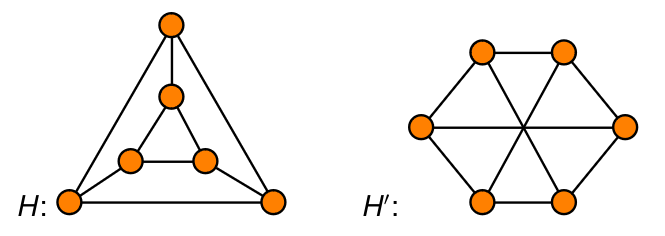
\includegraphics[width=0.35\textwidth]{img/no_isomorfi}
    \end{figure}
    Questi due grafi non sono isomorfi, ma ad esempio, la condizione relativa al grado dei veritici è vera. Andiamo ad analizzare i \textit{cicli}, attraverso le potenze delle matrici di adiacenza.

    \textbf{Proprietà}: si verifica che $\forall G = (V, E)$ e $\forall k \in \mathbb{N}$ con $k \geq 2$, la matrice $A^k$ (potenza $k$-esima della matrice di adiacenza) contiene nella posizione $(i, j)$ il numero di cammini in $G$ di lunghezza $k$ tra $v_i$ e $v_j$, e nella posizione $(i, i)$ il numero di cicli in $G$ di lunghezza $k$ contenenti $v_i$. Quindi, dalla diagonale principale di $A^k$ deduco se in $G$ sono presenti o no cicli di lunghezza $k$.
    
    {\centering
        \begin{minipage}[t]{0.45\textwidth}
            \centering
            $A_H = \left(\begin{array}{cccccc} 
                0 & 1 & 1 & 1 & 0 & 0 \\
                1 & 0 & 1 & 0 & 0 & 1 \\ 
                1 & 1 & 0 & 0 & 1 & 0 \\
                1 & 0 & 0 & 0 & 1 & 1 \\
                0 & 0 & 1 & 1 & 0 & 1 \\
                0 & 1 & 0 & 1 & 1 & 0
            \end{array}\right)$
        \end{minipage}
        \begin{minipage}[t]{0.45\textwidth}
            \centering
            $A_{H'} = \left(\begin{array}{cccccc} 
                0 & 1 & 0 & 1 & 0 & 1 \\
                1 & 0 & 1 & 0 & 1 & 0 \\
                0 & 1 & 0 & 1 & 0 & 1 \\
                1 & 0 & 1 & 0 & 1 & 0 \\
                0 & 1 & 0 & 1 & 0 & 1 \\
                1 & 0 & 1 & 0 & 1 & 0 \\
            \end{array}\right)$
        \end{minipage}
    \par}
    Facendo la potenza $k$-esima di queste matrici (imponiamo $k = 3$) abbiamo:

    {\centering
        \begin{minipage}[t]{0.45\textwidth}
            \centering
            $A_H^3 = \left(\begin{array}{cccccc}
                \mathbf{2} & 6 & 6 & 7 & 3 & 3 \\
                6 & \mathbf{2} & 6 & 3 & 7 & 3 \\
                6 & 6 & \mathbf{2} & 3 & 3 & 7 \\
                7 & 3 & 3 & \mathbf{2} & 6 & 6 \\
                3 & 7 & 3 & 6 & \mathbf{2} & 6 \\
                3 & 3 & 7 & 6 & 6 & \mathbf{2}
            \end{array}\right)$
        \end{minipage}
        \begin{minipage}[t]{0.45\textwidth}
            \centering
            $A_{H'}^3 = \left(\begin{array}{cccccc}
                \mathbf{0} & 9 & 0 & 9 & 0 & 9 \\
                9 & \mathbf{0} & 9 & 0 & 9 & 0 \\
                0 & 9 & \mathbf{0} & 9 & 0 & 9 \\
                9 & 0 & 9 & \mathbf{0} & 9 & 0 \\
                0 & 9 & 0 & 9 & \mathbf{0} & 9 \\
                9 & 0 & 9 & 0 & 9 & \mathbf{0} 
            \end{array}\right)$
        \end{minipage}
    \par}
    Dall'analisi delle \textit{potenze delle matrici di adiacenza} è evidente che a partire da ogni vertice in $H$ sono presenti due cicli di lunghezza 3 (in realtà si tratta dello stesso ciclo, ma percorso in direzioni opposte), mentre in $H'$ non esistono cicli di lunghezza 3. Questo prova che $H$ e $H'$ \textbf{non} sono \textbf{isomorfi}.
\end{flushleft}

\section{Grafi Planari}

\begin{flushleft}
    Un grafo $G = (V, E)$ si dice \textbf{planare} se esiste un'applicazione iniettiva, detta \textbf{immersione}, $i: |G| \mapsto \mathbb{R}^2$, dove $|G|$ è la realizzazione geometrica del grafo (a parole povere significa che rappresentando il grafo in due dimensioni non sono presenti deli incroci tra i suoi spigoli).
    \begin{boxA}
        \textcolor{orange}{\textbf{Esempio}}: $K_4$ è un \textit{grafo planare}, perché esiste una opportuna sua immersione (iniettiva) nel piano.

        \begin{center}
            \centering
            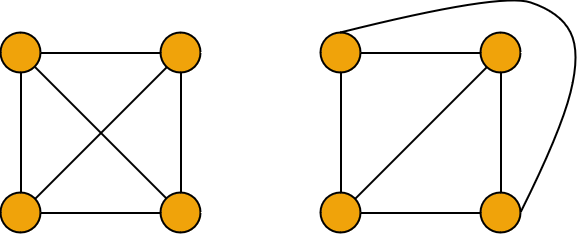
\includegraphics[width=0.25\textwidth]{img/k4}
        \end{center}
    \end{boxA}
\end{flushleft}

\newpage
\begin{flushleft}
    \textbf{Proprietà}: Il grafo $K_{3,3}$ \textbf{non} è \textbf{planare} (completo e bipartito).
    
    \begin{figure}[h]
        \centering
        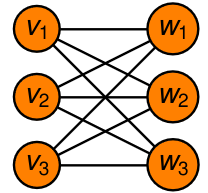
\includegraphics[width=0.15\textwidth]{img/k33}
    \end{figure}

    \textbf{Teorema della Curva di Jordan}: data in $\mathbb{R}^2$ una curva chiusa e semplice $\mathcal{C}$ essa divide $\mathbb{R}^2$ in due parti $\text{Int}\mathcal{C}$ e $\text{Ext}\mathcal{C}$, tali che $\forall a \in \text{Int}\mathcal{C}$ e $\forall b \in \text{Ext}\mathcal{C}$ ogni cammino continuo in $\mathbb{R}^2$ da $a$ a $b$ interseca la curva $\mathcal{C}$ (ovvero: per ogni applicazione continua $f: [0, 1] \mapsto \mathbb{R}^2$ tale che $f(0) = a$ e $f(1) = b$, si ha $f([0, 1]) \cap \mathcal{C} \neq \emptyset$)

    \begin{boxA}
        \textcolor{olive}{\textbf{Dimostrazione} ($K_{3,3}$ non è planare)}: poniamo $V(K_{3,3}) = \{a, b, c\} \cup \{u, v, w\}$ e supponiamo per \textbf{assurdo} che $K_{3,3}$ si \textit{immerga} nel piano. Consideriamo ora la curva $\mathcal{C}$ formata dal ciclo su $\{a, u, b, v\}$

        {\centering
            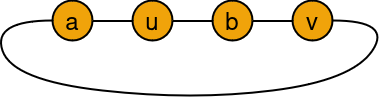
\includegraphics[width=0.25\textwidth]{img/k33_1}
        \par}
        Senza perdere di generalità, consideriamo il vertice $c \in \text{Int}\mathcal{C}$ (la curva $\mathcal{C}$ è definita dai vertici $\{a, v, b, u\}$) che si dovrà collegare sia a $u$ che a $v$:

        {\centering
            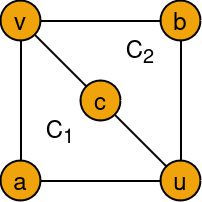
\includegraphics[width=0.15\textwidth]{img/k33_2}
        \par}
        Chiamiamo $\mathcal{C}_1$ la curva composta da $\{a, u, c, v\}$ e la curva $\mathcal{C}_2$ composta invece da $\{b, u, c, v\}$. Per posizionare $w$ ci sono tre possibilità: 
        \begin{enumerate}[nosep]
            \item $w \in \text{Int}\mathcal{C}_1$: in questo caso lo spigolo $\{w, b\}$, per il \textit{teorema della curva di Jordan}, deve intersecare $\mathcal{C}_1$ e quindi $K_{3,3}$ non può essere planare.
            \item $w \in \text{Int}\mathcal{C}_2$: in questo caso lo spigolo $\{w, a\}$, per il \textit{teorema della curva di Jordan}, deve intersecare $\mathcal{C}_2$ e quindi $K_{3,3}$ non può essere planare.
            \item $w \in \text{Ext}\mathcal{C}$: lo spigolo, in questo caso, per il \textit{teorema della curva di Jordan}, deve intersecare $\mathcal{C}$ e quindi $K_{3,3}$ non può essere planare
        \end{enumerate}
        Considerando tutti i casi, si giunge ad un \textbf{assurdo}, quindi $K_{3,3}$ non è planare.
    \end{boxA}
\end{flushleft}

\newpage
\begin{flushleft}
    \textbf{Proprietà}: il grafo $K_5$ \textbf{non} è \textbf{planare}

    \begin{figure}[h]
        \centering
        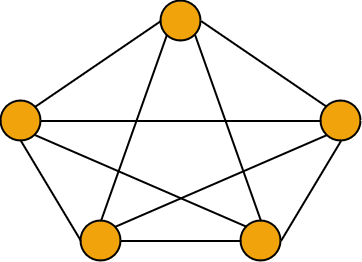
\includegraphics[width=0.25\textwidth]{img/k5}
    \end{figure}

    \begin{boxA}
        \textcolor{olive}{\textbf{Dimostrazione}}: procedimento analogo alla dimostrazione precendente, per \textbf{assurdo}, supponiamo che $K_5$ si immerga nel piano, disegnando i primi 3 vertici.

        \begin{center}
            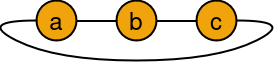
\includegraphics[width=0.25\textwidth]{img/k5_1}
        \end{center}
        Consideriamo ora un vertice $d \in V \; | \; d \in \text{I}\mathcal{C}$

        \begin{center}
            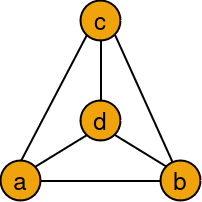
\includegraphics[width=0.15\textwidth]{img/k5_2}
        \end{center}
        Consideriamo ora le 3 curve: 
        \begin{enumerate}[nosep]
            \item $\mathcal{C}_1$ formata dai vertici: $\{a, b, d\}$
            \item $\mathcal{C}_2$ formata dai vertici: $\{a, c, d\}$
            \item $\mathcal{C}_3$ formata dai vertici: $\{b, c, d\}$
        \end{enumerate}
        E ricordiamo la presenza della curva $\mathcal{C}$ formata dai vertici $\{a, b, c\}$, per inserire il vertice $e$ ho 4 possibilità:
        \begin{enumerate}[nosep]
            \item $e \in \text{Int}\mathcal{C}_1$: lo spigolo $\{e, c\}$, per il \textit{teorema della curva di Jorda}, deve intersecare $\mathcal{C}_1$ e quindi $K_5$ non può essere planare.
            \item $e \in \text{Int}\mathcal{C}_2$: lo spigolo $\{e, b\}$, per il \textit{teorema della curva di Jorda}, deve intersecare $\mathcal{C}_2$ e quindi $K_5$ non può essere planare.
            \item $e \in \text{Int}\mathcal{C}_3$: lo spigolo $\{e, a\}$, per il \textit{teorema della curva di Jorda}, deve intersecare $\mathcal{C}_3$ e quindi $K_5$ non può essere planare.
            \item $e \in \text{Ext}\mathcal{C}$: lo spigolo $\{e, d\}$, per il \textit{teorema della curva di Jorda}, deve intersecare $\mathcal{C}$ e quindi $K_5$ non può essere planare.
        \end{enumerate}
        In tutti i casi, si giunge ad un \textbf{assurdo}, quindi $K_5$ \textbf{non} è \textbf{planare}.
    \end{boxA}
\end{flushleft}

\newpage
\begin{flushleft}
    \textbf{Omeomorfismo}: due grafi $G$ e $G'$ si dicono \textit{omeomorfi} se è possibile passare dall'uno all'altro tramite una successione finita di operazioni del tipo:

    {\centering
        $\{u, v\} \leftrightarrow \{u, w\} \cup \{w, v\}$
    \par}

    \textbf{Teorema di Kuratowski (1930)}: un grafo è planare se e solo se non contiene sottografi omeomorfi a $K_{3,3}$ o a $K_5$.

    In pratica se un grafo $G = (V, E)$ contiene $K_5$ o $K_{3,3}$ allora \textbf{non} è un \textbf{grafo planare}.

    \textbf{Facce}: Se $G = (V, E)$ è un \textbf{grafo planare}, si dicono facce dell'immersione $i: |G| \mapsto \mathbb{R}^2$, o semplicemente facce di $G$, le componenti connesse di $\mathbb{R}^2 - i(|G|)$.

    Normalmente il numero di faccie viene indicato con $F$, per cui il numero delle facce è: $\# F$.

    \textbf{Albero} (o \textbf{tree}): è un grafo $G = (V, E)$ connesso e privo di cicli.

    \textbf{Foresta}: è un grafo $G = (V, E)$ privo di cicli, ma, eventualmente, con più componenti connesse.

    \textbf{Teorema di Caratterizzazione di Alberi}: sia $T = (V, E)$ un grafo. Sono equivalenti le seguenti affermazioni:
    \begin{enumerate}[nosep]
        \item $T$ è un \textbf{albero}.
        \item $\forall v, w \in V \; \exists! \; \text{cammino}$ in T che congiunge $v$ con $w$.
        \item $T$ è connesso e $\forall e \in E$ il grafo $T' = (V, E - \{e\})$ non è connesso.
        \item $T$ non presenta cicli e $\forall e \in \binom{V}{2} - E$ il grafo $T' = (V, E \cap {e})$ contiene almeno un ciclo.
    \end{enumerate}
    In particolare, la (3) significa che, se tolgo uno spigolo qualsiasi, il grafo diventa non connesso, mentre la (4) implica che, se aggiungo uno spigolo tra vertici esistenti, allora sicuramente il grafo presenterà almeno un ciclo, perché per ogni vertice che aggiungo, aggiungo anche uno spigolo.

    \textbf{Teorema di Caratterizzazione di Alberi Finiti}: sia $T = (V, E)$ un grafo finito. $T$ è un \textbf{albero} \textit{se e solo se} $T$ è connesso e $\# V - 1 = \# E$ (tuttavia, si parte da 1 vertice con 0 spigoli, per questo il ``-1'').
\end{flushleft}

\newpage
\begin{flushleft}
    \textbf{Teorema di Eulero}: se $G = (V, E)$ è un grafo finito, planare e connesso, allora 
    
    {\centering
        $\# V - \# E + \# F = 2$
    \par}

    \begin{boxA}
        \textcolor{olive}{\textbf{Dimostrazione}}: dimostrazione per \textbf{induzione} su $\# F = f$ 

        {\centering
            \begin{minipage}[t]{0.45\textwidth}
                \centering
                \textbf{Hp.}: Grafo finito, planare e connesso
            \end{minipage}
            \begin{minipage}[t]{0.45\textwidth}
                \centering
                \textbf{Th.}: $\# V - \# E + \# F = 2$
            \end{minipage}
        \par}

        \textcolor{red}{\textbf{Passo Iniziale}} ($f = 1$) \\
        Se $f = 1$, il grafo è un albero. Quindi, vale che $\# V - 1 = \# E$, cioé $\# V - \# E = 1$, sommando $\# F$ da entrambi i lati otteniamo che:
        \begin{align*}
            \# V - \# E + \# F &= 1 + 1 \\
            &= 2
        \end{align*}

        \textcolor{red}{\textbf{Passo Induttivo}}:
        \begin{center}
            \begin{minipage}[t]{0.45\textwidth}
                \centering
                \textbf{Hp.} \\
                La formula di Eulero vale per tutti i grafi finiti, planari e connessi con $F - 1$ facce.
            \end{minipage}
            \begin{minipage}[t]{0.45\textwidth}
                \centering
                \textbf{Th.} \\
                Vale anche $F$ facce.
            \end{minipage}
        \end{center}

        Considero $G = (V, E)$ grafo finito, planare e connesso con $f \geq 2$ facce, essendoci almeno 2 facce, sicuramente $G$ non è un albero. Non essendo albero, per $G$ non valgono le proprietà degli alberi, in particolare la (3): $\exists \overline{e} \in E \; | \; G' = (V, E - \{e\})$, quindi rimane connesso. 

        Osservo che $G'$ è finito, planare e connesso, inoltre $G'$ ha $f-1$ facce in quanto togliendo $e$ ho fuso due facce; per ipotesi induttiva, la formula vale per $G': \# V' - \# E' + \# F = 2$, ma:

        {\centering
            $\# V' - \# E' + \# F = \# V - (\# E - \cancel{1}) + (\# F - \cancel{1}) = 2$
        \par}
        quindi la formula rimane valida.
    \end{boxA}

    \textbf{Corollario}: se $G = (V, E)$ è un grafo finito, planare e connesso, allora esiste almeno un vertice $v$ tale che $deg(v) \leq 5$
    \begin{boxA}
        \textcolor{olive}{\textbf{Dimostrazione}}: ogni faccia ha almeno 3 lati ed ogni spigolo ha almeno 2 facce, quindi: $\# E \geq \frac{3 \cdot \# F}{2}$, ovvero $\# F \leq \frac{2 \cdot \# E}{3}$.

        Sostituendolo nella \textit{formula di Eulero} ottendo:

        {\centering
            $2 = \# V - \# E + \# F \leq \# V - \# E + \frac{2 \cdot \# E}{3} = \# V - \frac{\# E}{3}$
        \par}
        Per \textbf{assurdo}, suppongo che il grado di $v \geq 5$, ma poiché $\underset{v \in V}{\sum} deg(v) = 2 \cdot \# E$, segue che $2 \cdot \# E \geq 6 \cdot \# V$, ovvero che $\# E \geq 3 \cdot \# V$. Ma questo significherebbe che $3 \cdot \# V \leq \# E \leq 3 \cdot \# V - 6$ che è \textbf{assurdo}.
    \end{boxA}
\end{flushleft}

\newpage
\begin{flushleft}
    \textbf{Corollario}: se $G = (V, E)$ è un grafo finito, planare e connesso con $\# V < 12$, allora esiste ameno un vertice $v$ tale che $deg(v) \leq 4$

    \begin{boxA}
        \textcolor{olive}{\textbf{Dimostrazione}}: supponiamo che $deg(v) \geq 5$, allora avremo che $2 \cdot \# E \geq 5 \cdot \# V \; \rightarrow \; \frac{5}{2} \# V \leq \# E$. Per la conseguenza della \textit{formula di Eulero} abbiamo che $\# E \leq 3 \cdot \# V - 6$ 

        {\centering
            $5 \cdot \# V \leq 6 \cdot \# V - 12 \; \Rightarrow \; \# V \geq 12$
        \par}
        che è un \textbf{assurdo}.
    \end{boxA}

    \textbf{Solidi Platonici}: tramite la formula di Eulero per i grafi planari, si dimostr anche l'esistenza di soli 5 solidi platonici: poliedri semplici regolari sulle facce, sugli spigoli e sui vertici.

    \begin{figure}[h]
        \centering
        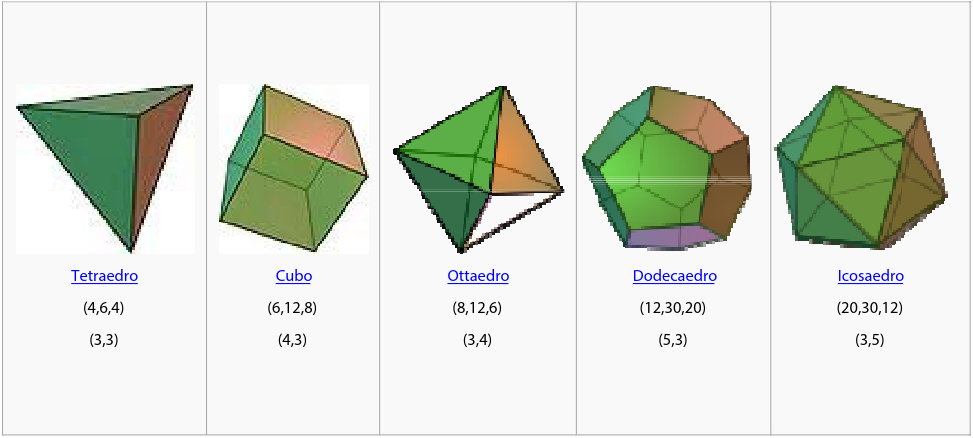
\includegraphics[width=0.75\textwidth]{img/solidi_platonici}
    \end{figure}
    La tabella indica per ogni solido platonico la terna $(F, S, V)$ ed una coppia $(N, M)$, con $N$ pari al numero di lati di ogni faccia e $M$ pari al numero di spigoli su ogni vertice (cioè la sua valenza). Cubo e ottaedro sono duali, dodecaedro e icosaedro sono duali. Il tetraedro è duale a se stesso (la dualità inverte le terne e le coppie di numeri nella tabella).
\end{flushleft}

\newpage
\section{Spanning Tree}
\begin{flushleft}
    \textbf{Spanning Tree}: sia $G = (V, E)$ un grafo. Un sottografo $T$ di $G$ si dice \textit{spanning tree} o \textbf{albero di copertura} se $T$ è un albero e se $V(G) = V(T)$.

    \textbf{N.B.} se $G$ ammette un albero di copertura, $G$ è sicuramente connesso.
    \begin{boxA}
        \textcolor{olive}{\textbf{Dimostrazione}}: consideriamo l'insieme $\mathcal{C}$ dei sottografi $C$ del grafo principale $G$ che hanno $V(G) = V(C)$
        \begin{itemize}[nosep]
            \item sicuramente $\mathcal{C}$ è non nullo. Quindi esisterà un sottografo $\overline{C} \; | \; \# E(\overline{C}) \leq \# E(C) \; \forall C \in \mathcal{C}$, cioé prendiamo il sottografo minimale (col minimo numero di spigoli), ma allora $\overline{C}$ è un albero.
            \item supponiamo per \textbf{assurdo} che non lo fosse, allora esisterebbe uno spigolo $e \in E(\overline{C})$ tale che, senza di esso, il grafo sarebbe comunque connesso, significherebbe che questo nuovo sottografo apparteneva a $\mathcal{C}$, con un numero minore di spigoli, il che è \textbf{assurdo}.
        \end{itemize}
    \end{boxA}

    \textbf{Caratterizzazione dei Grafi Bipartiti}: condizione \textbf{necessaria} e \textbf{sufficiente} affinché un grafo $G$ sia bipartito è che $G$ sia privo di cicli di lunghezza dispari.

    \begin{boxA}
        \textcolor{olive}{\textbf{Dimostrazione}} \newline
        \textcolor{red}{\textbf{Prima Parte}} ``$\Rightarrow$'' \\
        Se provo a disegnere un ciclo di lunghezza dispari, assegnando alternativamente i vertici, mi rimane l'ultimo fuori. \\
        \textcolor{red}{\textbf{Seconda Parte}} ``$\Leftarrow$'' \\
        \textbf{Hp.}: $G$ connesso e non contiene cicli di lunghezza dispari. \\
        Essendo connesso, esiste sicuramente uno spannig tree, quindi, posso scegliere un vertice e nominarlo $r$ (radice) ora considero:
        \begin{itemize}[nosep]
            \item $V' = \{v \in V \; | \; \text{il cammino in } T \text{ da } r \text{ a } v \text{ ha lunghezza pari}\}$.
            \item $V'' = \{v \in V \; | \; \text{il cammino in } T \text{ da } r \text{ a } v \text{ ha lunghezza dispari}\}$
        \end{itemize}
        Rimane da provare che, $\forall e \in E$, i suoi estremi $w'$ e $w''$ sono tali che $w' \in V'$ e $w'' \in V''$ (o viceversa).
        \begin{itemize}[nosep]
            \item se uno spigolo $e \in E(T)$ appartiene all'albero.
            \item se uno spigolo $e \not\in E(T)$ non appartiene all'albero, significa che chiude un ciclo, ma se i due estremi fossero nella stessa classe, avrebbero lunghezza dispari. Contro l'ipotesi.
        \end{itemize}
    \end{boxA}
\end{flushleft}

\newpage
\section{Colorazioni di Grafi}
\begin{flushleft}
    \textbf{Colorazione sui vertici}: dato un grafo $G$, si dice \textit{colorazione} (sui vertici) un'applicazione $f: V \mapsto C$, ove $C$ è un'insieme (detto ``insieme dei colori'') ed $f$ è tale che $\forall e = \{v, w\} \in E$ si ha $f(v) \neq f(w)$, in pratica, ogni volta che  vertici sono collegati da uno spigolo, devono essere di colori diversi.

    \textbf{Numero Cromatico}: si definisce \textit{numero cromatico} di un grafo $G$, il minimo numero di colori tale per cui $\exists f: V \mapsto C$ colorazione, ovvero:

    {\centering
        $\mathcal{X}(G) = \min \{\# C \; | \; \exists f: V \mapsto C, \; f \; \text{colorazione}\}$
    \par}
    \textbf{Proprietà}:
    \begin{itemize}[nosep]
        \item $\mathcal{X}(G) = 1$ se e solo se $E(G) = \emptyset$
        \item $\mathcal{X}(G) = 2$ se e solo se $G$ è \textbf{bipartito}.
        \item $\mathcal{X}(K_n) = n \; \forall n \in \mathbb{N}$
        \item se $G'$ è un sottografo di $G$, allora $\mathcal{X}(G') \leq \mathcal{X}(G)$
    \end{itemize}

    \textbf{Clique}: dato un grafo $G$ si dice \textit{clique} in $G$ un sottografo di $G$ isomorfo ad un grafo completo.
    
    \textbf{Numero di Clique}: dato un grafo $G$ si dice \textit{numero di clique} di $G$ (e si indica con $\omega(G)$) la massima cardinalità di un insieme di vertici di $G$ il cui sottografo indotto sia \textbf{clique} in $G$:

    {\centering
        $\omega(G) = \max \{\# K \; | \; K \subseteq V, \; \binom{V}{2} \subseteq E\}$
    \par}
    \textbf{Proprietà}: $\mathcal{X}(G) \geq \omega(G), \; \forall G$ grafo, ovvero, per colorare un grafo servono almeno $\omega(G)$ colori.

    Nel caso di grafi planari, il problema del calcolo di $\mathcal{X}(G)$ equivale al problema della \textit{colorabilità} delle cartine geografiche.

    \textbf{Teorema dei Quattro Colori} ([Apple e Hacken, 1977], venne dimostrato tramite l'utilizzo di un computer): ogni \textbf{grafo planare} è $4$-colorabile:

    {\centering
        $\mathcal{X}(G) \leq 4, \; \forall G \; \text{planare}$
    \par}
    senza l'appoggio di un computer viene dimostrato il risultato più debole:

    \textbf{Teorema dei Cinque Colori}: ogni ogni \textbf{grafo planare} è $5$-colorabile: $\mathcal{X}(G) \leq 5, \; \forall G \; \text{planare}$

    \begin{boxA}
        \textcolor{olive}{\textbf{Dimostrazione}}: suppongo di avere un grafo finito e planare (connesso). L'ipotesi di connessione non serve, in quanto posso considerare la componente connessa che richiede pià colori, risolvendo automaticamente di conseguenza le altre. \\
        Procediamo per \textbf{induzione} sull'ordine del grafo $\# V = n$ \\
        \textcolor{red}{\textbf{Passo Iniziale}}: se $n \leq 5$, il teorema è banale (coloro ogni vertice con un colore diverso)
    \end{boxA}
    \begin{boxA}
        \textcolor{red}{\textbf{Passo Induttivo}}: supponiamo che il teorema valga per tutti i grafi con $n-1$ vertici, noi lo vogliamo dimostrare per tutti i grafi con $n$ vertici. \\
        Poiché $G$ è finito, planare e connesso, per la \textit{formula di Eulero} $\exists \overline{v} \in V$ con $deg(\overline{v}) \leq 5$. Consideriamo il caso perggiore ($deg(\overline{v}) = 5$ e colorazione dei veritici adiacenti tutte diverse) e cancelliamo gli spigoli dei vertici adiacenti ad esso (chiameremo questo grafo $G'$):

        \begin{center}
            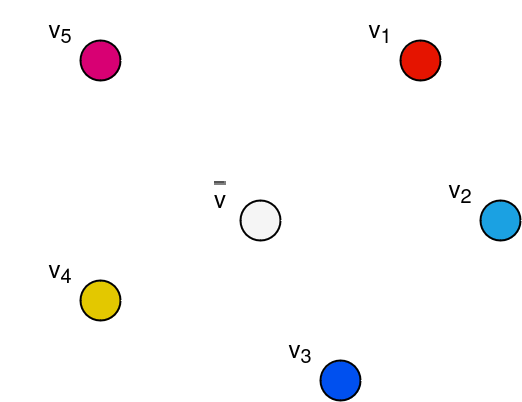
\includegraphics[width=0.3\textwidth]{img/5colori}
        \end{center}
        Consideriamo il sottografo di $G'$ indotto dai vertici colorati con $c_1$ e $c_3$ (colorazione del vertice $v_3$) e $c_3$ che chiameremo $H_{1, 3}$. Abbiamo due casi:
        \begin{enumerate}[nosep]
            \item supponiamo che $v_3$ non appartenga alla stessa componente connessa che contiene $v_1$, in questo caso posso scambiare i colori $c_1$ e $c_3$ della componente connessa di $v_1$. Ottenendo una colorazione di $G'$ nella quale i vertici adiacenti a $\overline{v}$ non usano il colore $c_1$
            
            {\centering
                Assogno a $\overline{v}$ il colore $c_1$, ottenendo la colorazione cercata di $G$ di 5 colori.
            \par}
            \item supponiamo ora che $v_1$ e $v_3$ appartengano alla stessa componente connessa di $H_{1, 3}$. In tal caso, essite un cammino in $G'$ di vertici alternativamente colorati con $c_1$ e $c_3$ che collega $v_1$ e $v_3$, se a tale cammino aggiungo spigoli in $G$ $\{\overline{v}, v_1\}$ e $\{\overline{v}, v_2\}$, ottengo una curva chiusa semplice $\mathcal{C}$ del piano, in particolare $v_2 \in \text{Int}\mathcal{C}$ e $v_4 \in \text{Ext}\mathcal{C}$, quindi i vertici $v_2$ e $v_4$ non possono essere connessi da uno spigolo (si perderebbe l'ipotesi di planarità) e $\overline{v}$ può assumere o $c_2$ o $c_4$
        \end{enumerate}
        Considero ora il sottografo $G'$ indotto dai vertici colorati con $c_2$ e $c_4$ e lo chiamo $H_{2, 4}$. Anche qui abbiamo due casi:
        \begin{enumerate}[nosep]
            \item supponiamo che $v_4$ non appartenga alla stessa componente connessa che continene $v_2$, allora come a prima, posso scambiare i colori $c_2$ e $c_4$ della componente connessa con $v_2$, ottenendo una colorazione di $G'$ in cui i vertici adiacenti a $\overline{v}$ non usano il colore $c_2$

            {\centering
                Assegno a $\overline{v}$ il colore $c_2$, ottenendo la colorazione cercata di $G$ con 5 colori.
            \par}
            \item supponiamo invece che $v_2$ e $v_4$ appartengano alla stessa componente connessa, se ciò fosse possibile, esisterebbe un cammino $G'$ da $v_2$ a $v_4$ con vertici colorati alternativamente con $c_2$ e $c_4$. Per il \textit{teorema della curva di Jordan}, tale cammino dovrebbe intersecare la curva $\mathcal{C}$, ma il vertice di intersezione dovrebbe avere colore $\overline{c} \in \{c_1, c_3\}$ e contemporaneamente anche $\overline{c} \in \{c_2, c_4\}$, che è \textbf{assurdo}.
        \end{enumerate}
    \end{boxA}

    \textbf{Polinomio Cromatico}: dato un grafo $G = (V, E)$ ed un intero non negativo $t$, sia $p(G, t)$ la funzione che restituisce il numero di modi in cui è possibile colorare $G$ con un insieme di $t$ colori. Si dimostra che $p(G, t)$ è sempre un polinomio a coefficienti interi nella indeterminata $t$; $p(G, t)$ prende il nome di \textit{polinomio cromatico} del grafo $G$. \textbf{Proprietà}:
    \begin{boxA}
        \textcolor{orange}{\textbf{Esempi}} \\
        Un grafo con un vertice è colorabile in $t$ modi. \\
        Un grafo con due vertici è colorabile in $t^2$ modi. \\
        $I_n \; \rightarrow \; p(I_n, t) = t^n$ \\
        $P_2 \; \rightarrow \; p(P_2, t) = t(t-1)$ \\
        $P_3 \; \rightarrow \; p(P_3, t) = t(t-1)(t-1) = t(t-1)^2$ \\
        $P_n \; \rightarrow \; p(P_n, t) = t(t-1)^{n-1}$ \\
        $C_3 = K_3 \; \rightarrow \; p(K_3, t) = t(t-1)(t-2)$ \\
        $K_4 \; \rightarrow \; p(K_4, t) = t(t-1)(t-2)(t-3)$ \\
        $K_n \; \rightarrow \; p(K_n, t) = t(t-1) ... (t-n+1) = \frac{t!}{(t-n)!} \; \rightarrow \; D_{t, n}$ || disposizioni semplici
    \end{boxA}
    \textbf{Proprietà}:
    \begin{itemize}[nosep]
        \item non tutti i polinomi interi nella indeterminata $t$ sono polinomi cromatici di un grafo $G$
        \begin{itemize}[nosep]
            \item il polinomio cromatico ha termine noto nullo, per ogni grafo contenente almeno un vertice: $p(G, 0) = 0 \; \forall G = (V, E), \; \text{con} \; V \neq \emptyset$
            \item se $G$ contiene almeno uno spigolo, $p(G, t)$ è un polinomio divisibile per $(t-1)$: 
            
            {\centering
                $p(G, t) = 0, \; \forall G = (V, E), \; \text{con} \; E \neq \emptyset$
            \par}
        \end{itemize}
        \item se un grafo non è connesso, il polinomimo cromatico è il prodotto dei polinomi cromatici delle singole componenti connesse:

        {\centering
            $p(G, t) = p(G_1, t) \cdot p(G_2, t) \cdot ... \cdot p(G_m, t)$ \\
            con $G_1, G_2, ..., G_m$ le componenti connesse di $G$
        \par}
    \end{itemize}
    \begin{boxA}
        \textcolor{orange}{\textbf{Esempio}}: grafo ciclo $C_4$
        
        {\centering
            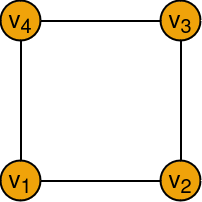
\includegraphics[width=0.15\textwidth]{img/c4}
        \par}
        \begin{itemize}[nosep]
            \item $v_1: \; t$ modi possibili
            \item $v_2: \; t-1$ modi possibili
            \item due casi possibili:
            \begin{itemize}[nosep]
                \item $v_1$ e $v_3$ hanno lo stesso colore: $t(t-1) \cdot 1 \cdot (t-1) = t(t-1)^2$
                \item $v_1$ e $v_3$ hanno colori diversi: $t(t-1)(t-2)(t-2) = t(t-1)(t-2)^2$
            \end{itemize}
        \end{itemize}
        Essendo due casi disgiunti si applica il principio della somma:

        {\centering
            $p(C_4, t) = t(t-1)^2 + t(t-1)(t-2)^2$
        \par}
        \textbf{N.B.} il polinomio cromatico ha sempre grado $n$ (numero dei vertici)
    \end{boxA}

    \textbf{Teorema di Whitney}: dato un grafo $G = (V, E)$ si fissi un ordinamento nell'insieme $E$ degli spigoli. Si dice \textbf{ciclo spezzato} in $G$ un sottografo di $G$ ottenuto da un ciclo in $G$ cancellando lo spigolo maggiore secondo l'ordinamento fissato. Allora:

    {\centering
        $p(G, t) = \underset{k \in \mathbb{N}_n}{\sum}(-1)^{n-k} \alpha_{n,k}t^k$
    \par}
    dove $n = \# V$ è l'ordine del grafo, $\alpha_{n,k}$ è il numero di sottoinsieme di $E$ di cardinalità $n-k$ che non contengono cicli spezzati.
    
    In pratica, si prende l'insieme degli spigoli, dandogli un ordine. Successivamente si considerano i \textbf{cicli spezzati}: prendendo tutti i cicli, si toglie lo spigolo più grande nell'ordinamento fissato ed infine, si applica la formula, dove $\alpha_{n,k}$ indica il numero di sottoinsiemi di $E$ con cardinalità $n-k$, che non contengono cicli spezzati.
    \begin{boxA}
        \textcolor{orange}{\textbf{Esempio}}: grafo ciclo $K_3$
        
        {\centering
            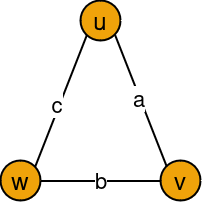
\includegraphics[width=0.15\textwidth]{img/k3}
        \par}
        Fisso l'ordinamento degli spigoli $a < b < c$, quindi l'unico ciclo spezzato è $\{a, b\}$, applico il \textit{teorema di Whitney}:

        {\centering
            $p(K_3, t) = \underset{k \in \mathbb{N}_3}{\sum} (-1)^{3-k} \cdot \alpha_{3,k} \cdot t^k = \alpha_{3,1}t - \alpha_{3,2}t^2 + \alpha_{3,3}t^3$ \\
            
            $\alpha_{3,1} = \# \{ \cancel{\{a, b\}}, \{b, c\}, \{c, a\} \} = 2 \quad \alpha_{3,2} = \# \{ \{a\}, \{b\}, \{c\} \} = 3 \quad \alpha_{3,3} = \# \{\emptyset\} = 1$ \\

            $p(K_3, t) = 2t + 3t^2 + t^3 = t(t-1)(t-2)$
        \par}
    \end{boxA}
\end{flushleft}

\section{Grafi Euleriani e Hamiltoniani}
\begin{flushleft}
    Problema dei ponti di \textbf{Konigsberg}: città natale di Eulero, contenente 7 ponti. Eulero si chiese se fosse possibile determinare un modo per percorrere tutti i ponti una sola volta e ritornare nel punto di partenza.

    \begin{figure}[h]
        \centering
        \begin{minipage}[t]{0.45\textwidth}
            \centering
            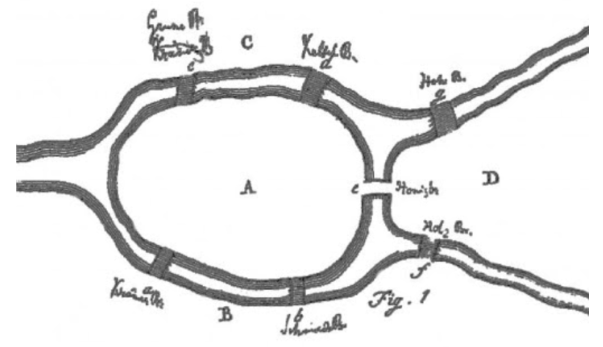
\includegraphics[width=\textwidth]{img/kon_1}
            \caption{Problema di Konigsberg}
        \end{minipage}
        \begin{minipage}[t]{0.45\textwidth}
            \centering
            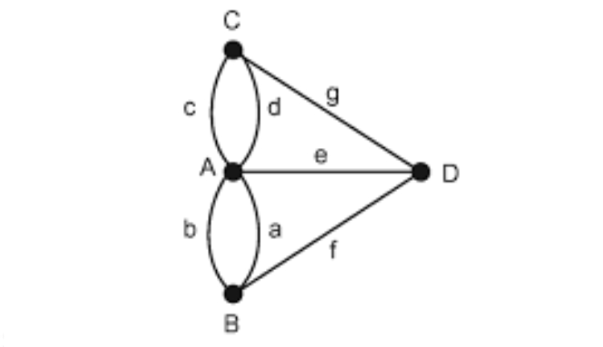
\includegraphics[width=\textwidth]{img/kon_2}
            \caption{Traduzione in grafi del problema}
        \end{minipage}
    \end{figure}
    \textbf{N.B.}: si noti che il grafo associato è un \textbf{multigrafo}. Le nozioni seguenti di teoria dei grafi sono valide anche nell'ambito esteso ai multigrafi.

    \begin{itemize}[nosep]
        \item \textbf{passeggiata}: dato un grafo $G = (V, E)$ si dice \textit{passeggiata} in $G$ una successione finita di vertici e spigoli consecutivi adiancenti:

        {\centering
            $u_0, e_1, u_1, e_2, ..., u_{k-1}, e_k, u_k$
        \par}
        dove $u_i \in V$, $e_i \in E$ ed $e_i = \{u_{i-1}, u_i\} \; \forall i \in \mathbb{N}_k$. Se $u_0 = u_k$, la passeggiata si dice \textbf{chiusa}. Si noti che un cammino in $G$ è una passeggiata in cui sono coinvolti vertici e spigoli tutti distanti (a parte il caso del ciclo, in cui vertice iniziale e vertice finale coincidano)
        \item \textbf{passeggiata elementare}: dato un grafo $G = (V, E)$, una passeggiata in $G$ si dice \textbf{elementare} se non contiene mai due volte lo stesso spigolo [passeggiata con spigoli tutti distinti (percorsi una sola volta)].
        \item \textbf{passeggiata semplice}: dato un grafo $G = (V, E)$, una passeggiata in $G$ si dice \textbf{semplice} se non visita mai due volte lo stesso vertice (a parte il caso in cui sia chiusa, in cui vertice iniziale e vertice finale coincidono).
        \item \textbf{cammino hamiltoniano}: dato un grafo $G = (V, E)$, si dice \textit{cammino hamiltoniano} (\textbf{ciclo hamiltoniano} se è chiuso) in $G$ una passeggiata in $G$ che contiene tutti gli spigoli di $G$, una e sola volta.
        \item \textbf{cammino euleriano}; dato un grafo $G = (V, E)$, si dice \textit{cammino euleriano} (\textbf{ciclo euleriano} se è chiuso) in $G$ una passeggiata in $G$ che contiene tutti gli spigoli di $G$, una e una sola volta.
        \item \textbf{grafo hamiltoniano}: un grafo $G = (V, E)$ si dice \textit{grafo hamiltoniano} se continene almeno un ciclo hamiltoniano (passeggiata chiusa semplice).
        \item \textbf{grafo euleriano}: un grafo $G = (V, E)$ si dice \textit{grafo euleriano} se contiene almeno un ciclo euleriano (passeggiata chiusa elementare).
    \end{itemize}
    Nono sono note condizioni ``semplici'' per verificare se un dato grafo $G$ è hamiltoniano o no. Banalmente, condizione necessaria, ma non sufficiente, è che $G$ sia connesso, con vertici tutti di grado $\geq 2$; condizione sufficiente, ma non non necessaria, è invece che il grado di ogni vertice sia maggiore o uguale a $\frac{\# V(G)}{2}$ (\textbf{Teorema di Dirac})

    \textbf{Teorema di Eulero}: un grafo $G = (V, E)$ è euleriano se e solo se è connesso con vertici tutti di grado pari.

    \begin{boxA}
        \textcolor{olive}{\textbf{Dimostrazione}}
        \begin{enumerate}[nosep]
            \item da dimostrare: Se il grafo è euleriano, allora è connesso in cui ogni vertice ha grado pari. Che sia connesso è banale. Per quanto riguarda i vertici, invece, ogni vertice deve poter essere raggiunto con uno spigolo e deve collegarsi ad un altro vertice con uno altro spigolo, quindi avrà sempre bisogno di coppie di spigoli.
            \item dimostrazione

            \begin{center}
                \begin{minipage}[t]{0.45\textwidth}
                    \centering
                    \textbf{Hp.} grafo connesso e tutti i vertici di grado pari
                \end{minipage}
                \begin{minipage}[t]{0.45\textwidth}
                    \centering
                    \textbf{Th.} grafo euleriano
                \end{minipage}
            \end{center}
            
            \begin{itemize}[nosep]
                \item consideriamo una passeggiata elementare di lughezza massima nel grafo: $W = u_0, e_1, u_1, e_2, ..., u_{k-1}, e_k, u_k$. Dato che è di lunghezza massima e, per ipotesi, tutti i vertici devono essere di grado pari, ovvero $u_k = u_0$, perché se no avrebbero un solo spigolo, ma quindi la passeggiata è un ciclo (passeggiata chiusa).
                \item per dimostrare che questa passeggiata elementare chiusa è un ciclo euleriano, dobbiamo dimostrare che continene \textbf{tutti} gli spigoli. Supponiamo per assurdo che esista uno spigolo $\overline{e}$ non compreso nella passeggiata $W$, ma tale che (per la connessione del grafo) abbia un estremo in $W$, allora, sarebbe possibile costruire una passeggiata:

                {\centering
                    $W' = \overline{v}, \overline{e}, u_j, e_{j+1}, ..., u_k = u_0, e_1, u_1, ..., u_{j-1}, e_j, u_j$
                \par}
                che è più lunga di $W$, che contraddice l'ipotesi iniziale, provando così la tesi.
            \end{itemize}
        \end{enumerate}
    \end{boxA}
\end{flushleft}